In this section will be presented an overview of the user's interface of the \ac{CKB} system. The application, as previously discussed will be a web app, accessible from a desktop browser. The access from mobile will be enabled and the interface will be scaled appropriately.

\section{General Overview}

The image below shows a map of the pages accessible by Educators and Students.

\begin{figure}[H]
    \centering
    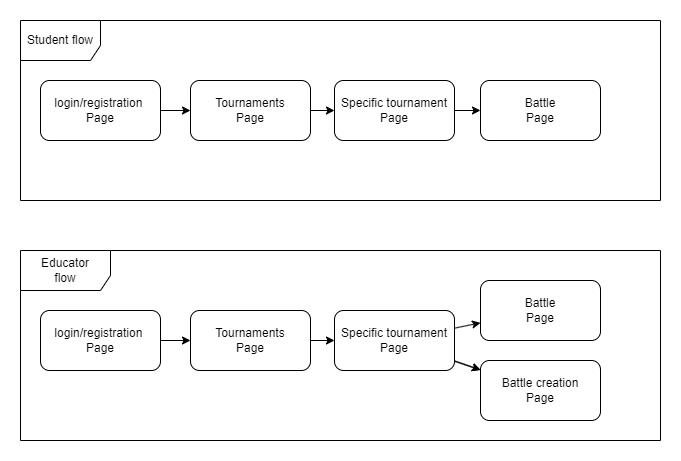
\includegraphics[width=0.95\linewidth]{misc//Images/flow.png}
    \caption{Web pages map}
    \label{fig:enter-label}
\end{figure}
\newpage
\subsubsection{Login Page}
This page is the first one viewed by the user when accessing the application. It contains two forms, one for the login of the user and one for the registration.
For the login the user can input their Username, password and select whether the user is an Educator or not.

For the registration the user is asked to insert their desired username, the password, and the type of user he desires to register as. Also the user has to insert the email where he will receive notification.

Once the user has created the account or logged into his own account he is directed to the tournaments page.

\begin{figure}[H]
    \centering
    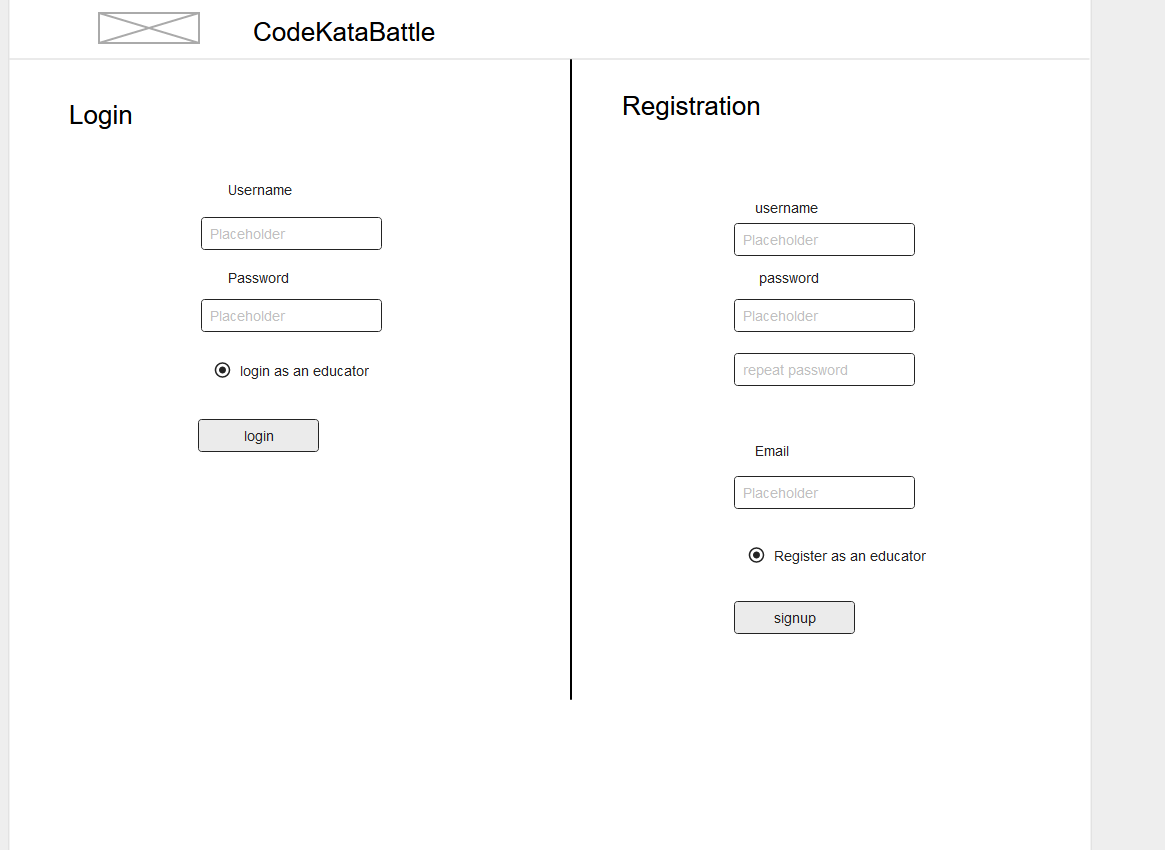
\includegraphics[width=1\linewidth]{misc//Images//UI Mockups/login.png}
    \caption{Login Page}
    \label{fig:enter-label}
\end{figure}
\newpage
\subsubsection{Main Page}
In this page a user can see the list of ongoing tournaments and the list of tournaments he/she is involved in, from which a specific tournament can be chosen to be redirected to.
If the user is an Educator then the page will also display a form for the creation of a tournament.

\begin{figure}[H]
    \centering
    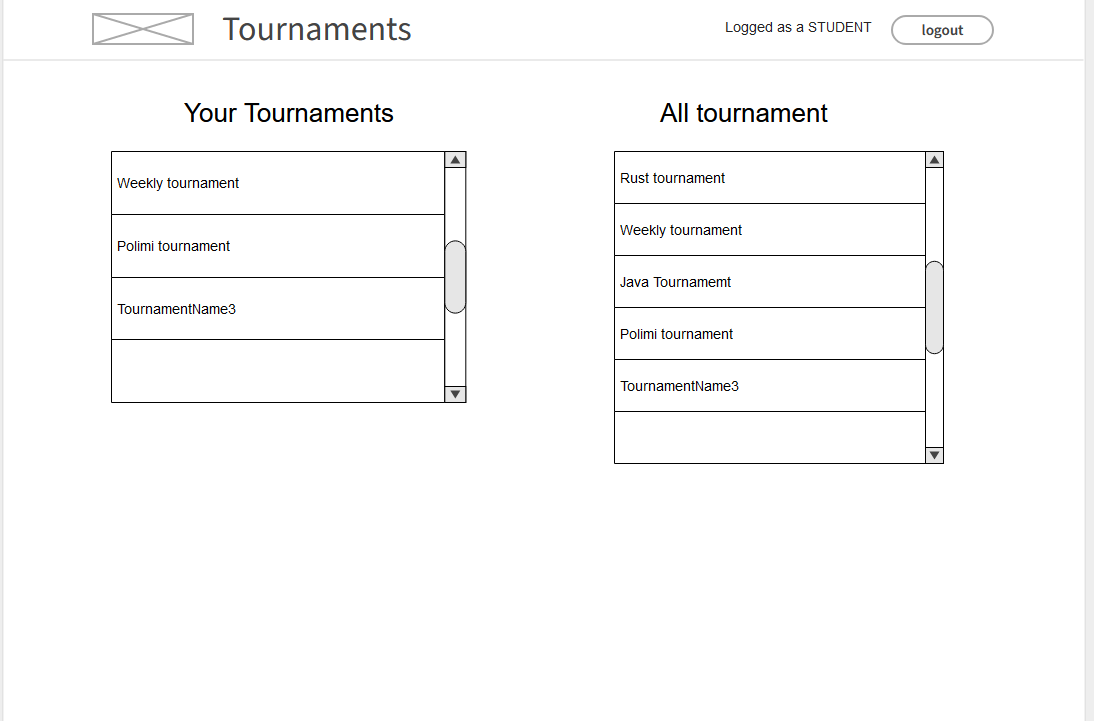
\includegraphics[width=0.8\linewidth]{misc//Images//UI Mockups/studMain.png}
    \caption{Student Main Page}
    \label{fig:enter-label}
\end{figure}


\begin{figure}[H]
    \centering
    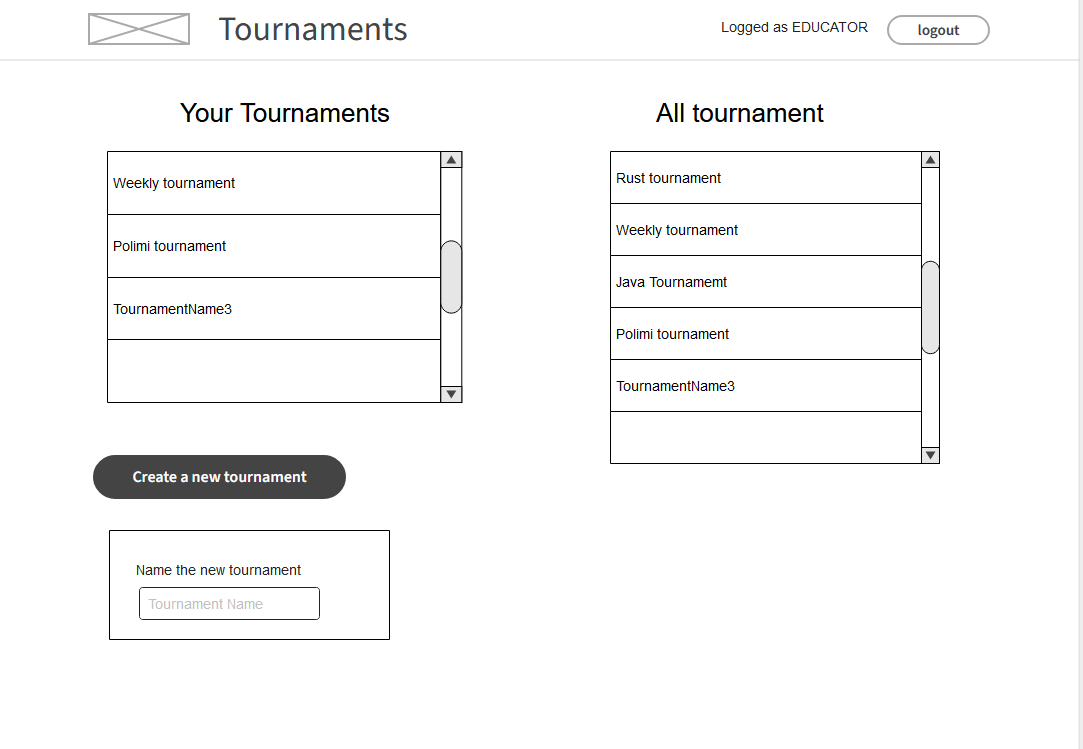
\includegraphics[width=0.8\linewidth]{misc//Images//UI Mockups/eduMain.png}
    \caption{Educator Main Page}
    \label{fig:enter-label}
\end{figure}

\newpage
\subsubsection{Tournament Page}
This page contains the list of battle in the context of the current tournament as well as the tournament leaderboard and 3 buttons.
The buttons allow the user to either create a battle in the tournament context, add a collaborator to the tournament or close the tournament.
The battles in the list can be selected to be directed to the selected battle page.
If the user is a student then instead of the three buttons there will be only one, allowing the student to join the tournament.

\begin{figure}[H]
    \centering
    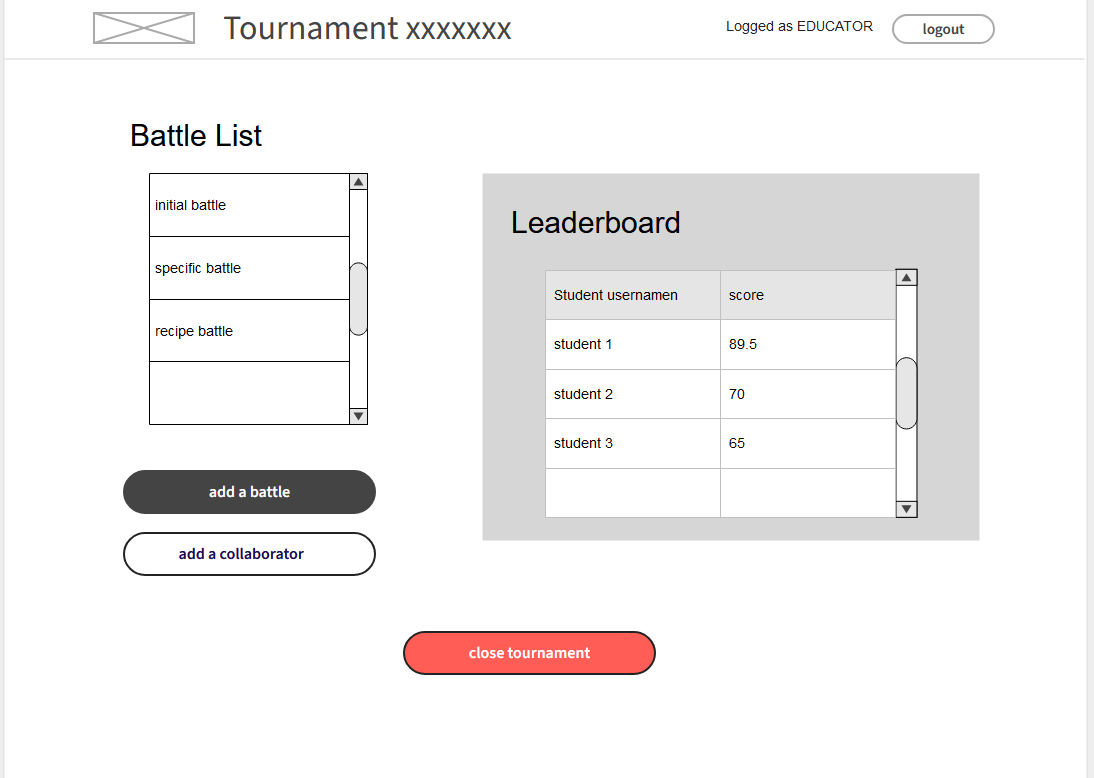
\includegraphics[width=0.7\linewidth]{misc//Images//UI Mockups/eduTournament.png}
    \caption{Educator Tournament Page}
    \label{fig:enter-label}
\end{figure}

\begin{figure}[H]
    \centering
    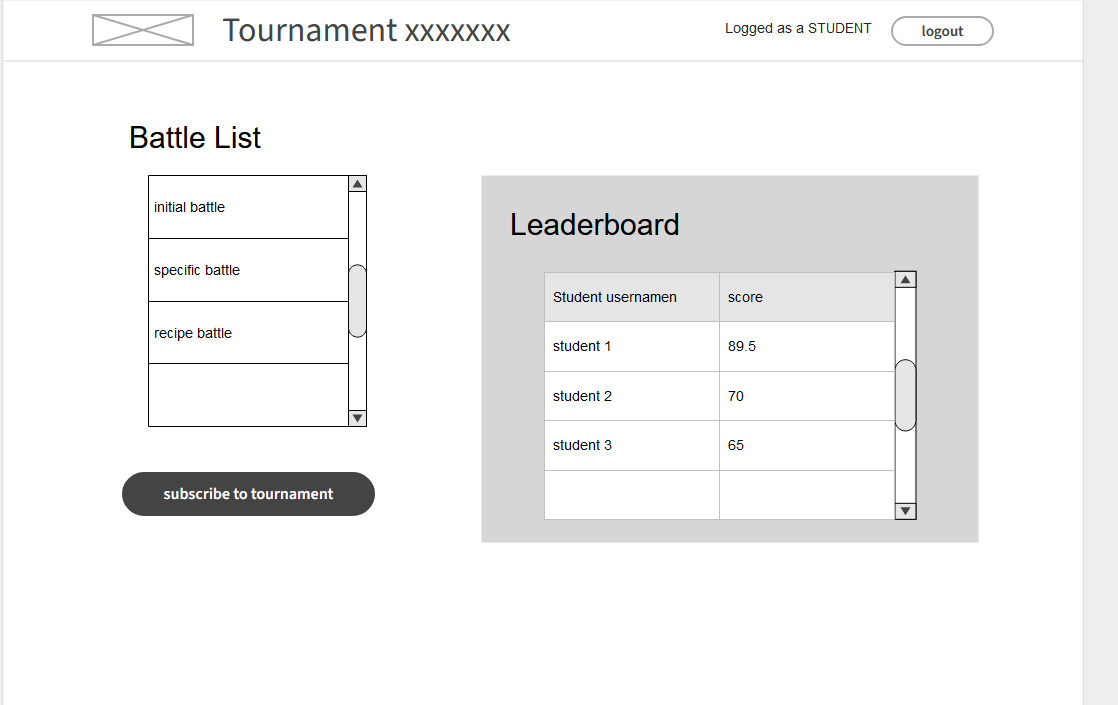
\includegraphics[width=0.7\linewidth]{misc//Images//UI Mockups/studTournament.png}
    \caption{Student Tournament Page}
    \label{fig:enter-label}
\end{figure}
\newpage
\subsubsection{Battle Creation Page}
The page presents a form where an educator can insert: 
\begin{itemize}
    \item Battle name;
    \item Text assignment for the \ac{CK}; 
    \item The two deadlines,
    \item The group rules.
\end{itemize}
There is also an upload form for the \ac{CK} testcases.

\begin{figure}[H]
    \centering
    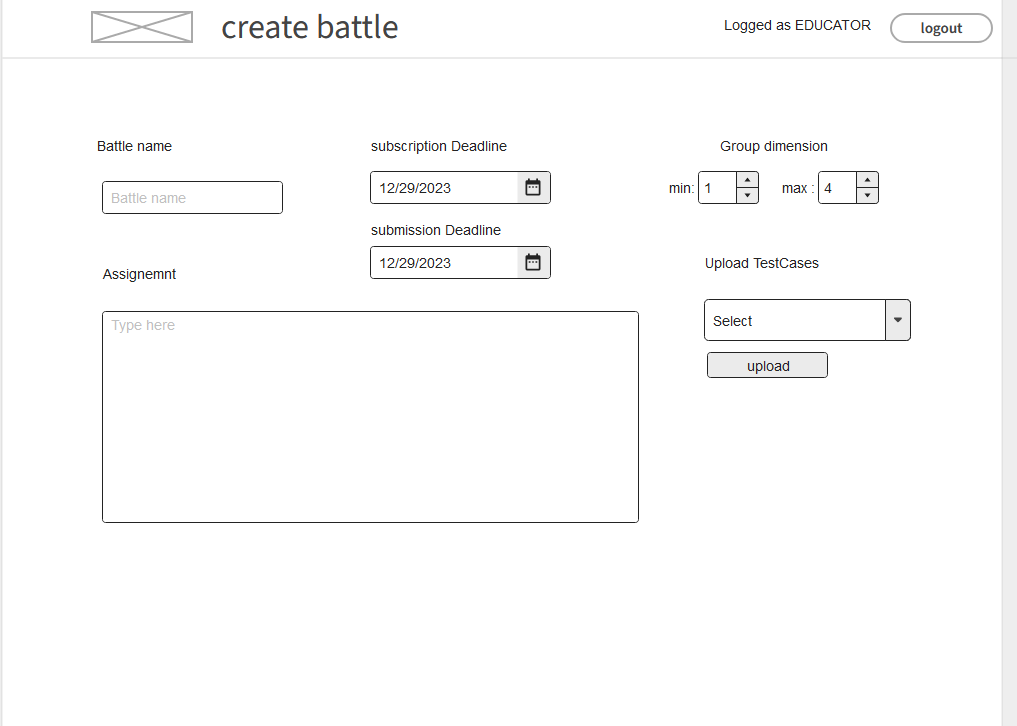
\includegraphics[width=1\linewidth]{misc//Images//UI Mockups/createBattle.png}
    \caption{Battle Creation}
    \label{fig:enter-label}
\end{figure}
\newpage
\subsubsection{Battle Page}
For both type of users the page presents the text of the assignment, the rules for the group size, the deadlines and finally the battle leaderboard.
In the student version during the battle subscription phase a button for joining the battle is present. When clicked the user is asked to insert a list of other student to join the battle with( following the group rules) in a form.

\begin{figure}[H]
    \centering
    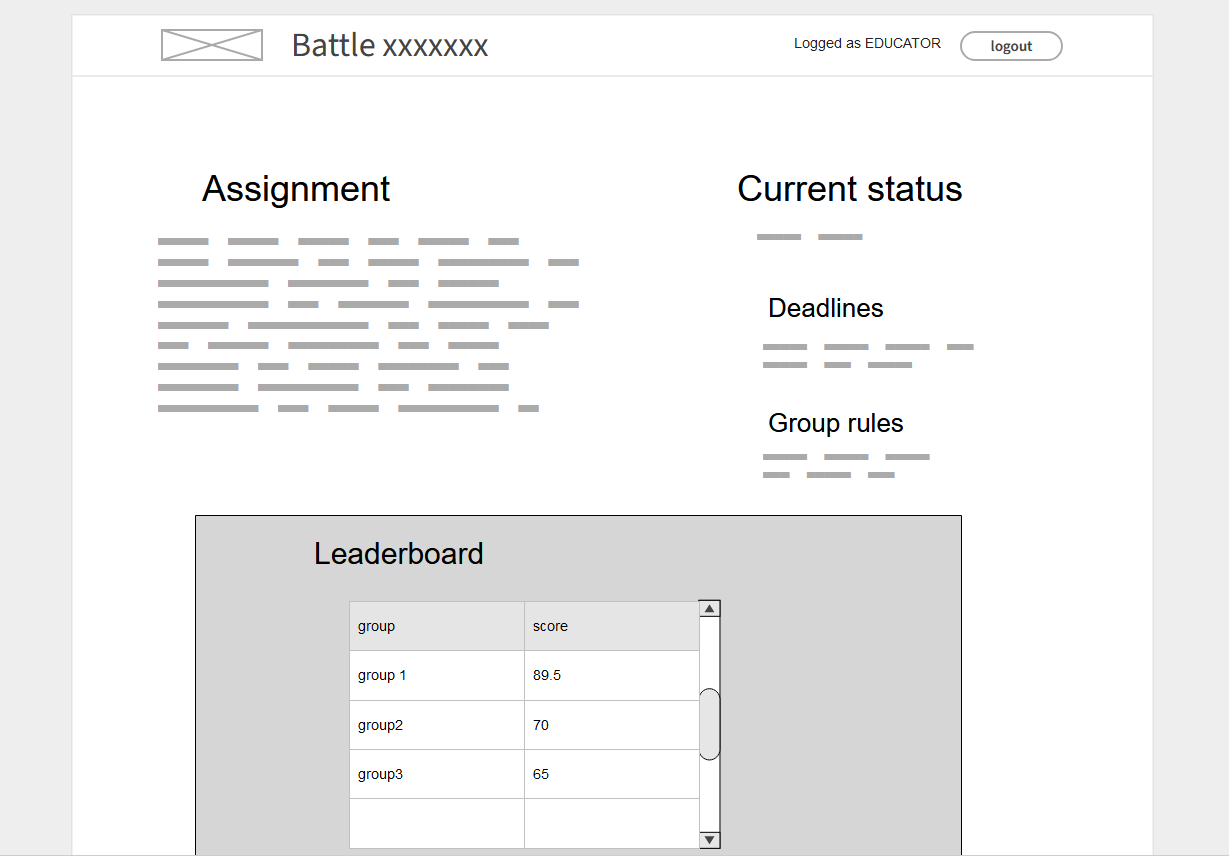
\includegraphics[width=1\linewidth]{misc//Images//UI Mockups/battle.png}
    \caption{Battle Page}
    \label{fig:enter-label}
\end{figure}
\newpage
\subsubsection{Manual Evaluation Page}

The page contains the source code of the group to be manually reviewed and an input where the user can put the decided score to be sent after clicking the 'score group' button.

\begin{figure}[H]
    \centering
    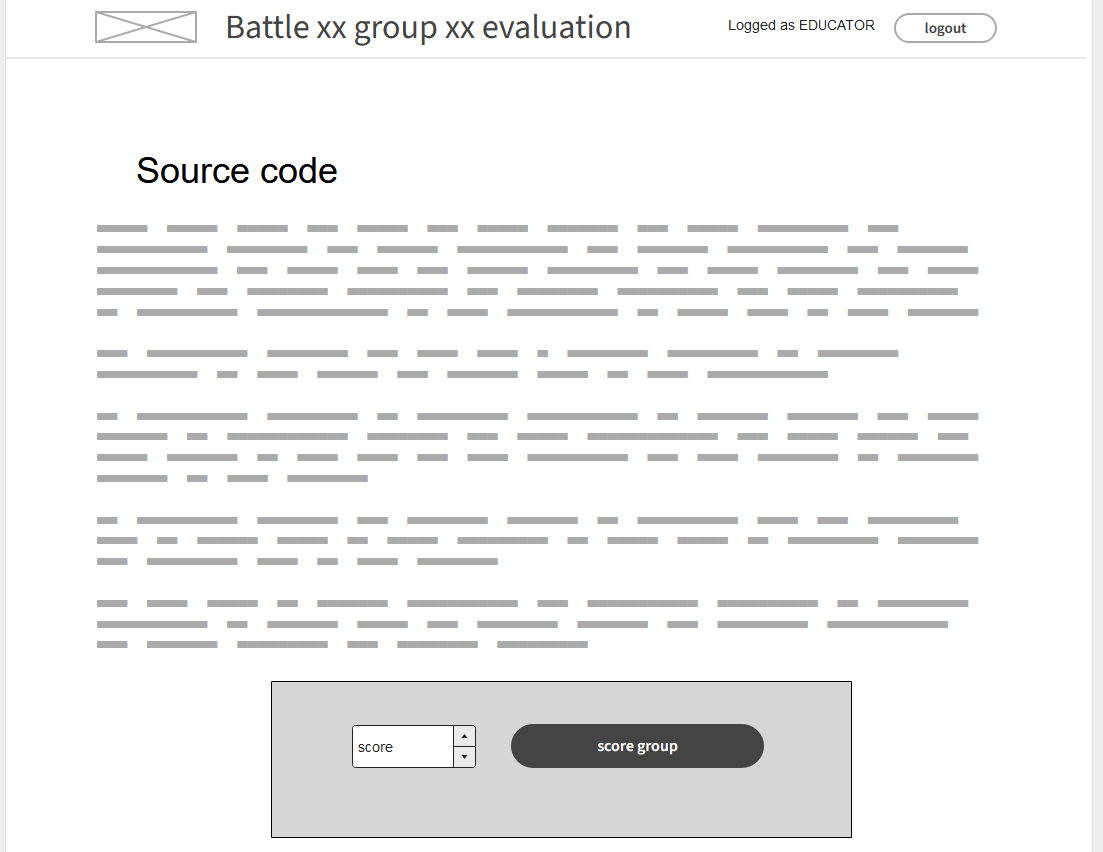
\includegraphics[width=1\linewidth]{misc//Images//UI Mockups/manualEval.png}
    \caption{Battle Page}
    \label{fig:enter-label}
\end{figure}